\documentclass{article}



\usepackage{arxiv}

\usepackage[utf8]{inputenc} % allow utf-8 input
\usepackage[T1]{fontenc}    % use 8-bit T1 fonts
\usepackage{hyperref}       % hyperlinks
\usepackage{url}            % simple URL typesetting
\usepackage{booktabs}       % professional-quality tables
\usepackage{amsfonts}       % blackboard math symbols
\usepackage{nicefrac}       % compact symbols for 1/2, etc.
\usepackage{microtype}      % microtypography
\usepackage{lipsum}		% Can be removed after putting your text content
\usepackage{float} % for [H] float placement
\usepackage{graphicx}
\usepackage{natbib}
\usepackage{doi}
\usepackage{tikz}
\usepackage{amsmath}



\title{An arbritary Lagrangian-Eulerian formulation for a non-Hertzian impact problem solved with variational methods}

%\date{September 9, 1985}	% Here you can change the date presented in the paper title
%\date{} 					% Or removing it

\author{ \href{https://orcid.org/0000-0000-0000-0000}{
\includegraphics[scale=0.06]{orcid.pdf}\hspace{1mm}David S.~Hippocampus}\thanks{Use footnote for providing further
		information about author (webpage, alternative
		address)---\emph{not} for acknowledging funding agencies.} \\
	Department of Computer Science\\
	Cranberry-Lemon University\\
	Pittsburgh, PA 15213 \\
	\texttt{hippo@cs.cranberry-lemon.edu} \\
	%% examples of more authors
	\And
	\href{https://orcid.org/0000-0000-0000-0000}{
\includegraphics[scale=0.06]{orcid.pdf}\hspace{1mm}Elias D.~Striatum} \\
	Department of Electrical Engineering\\
	Mount-Sheikh University\\
	Santa Narimana, Levand \\
	\texttt{stariate@ee.mount-sheikh.edu} \\
	%% \AND
	%% Coauthor \\
	%% Affiliation \\
	%% Address \\
	%% \texttt{email} \\
	%% \And
	%% Coauthor \\
	%% Affiliation \\
	%% Address \\
	%% \texttt{email} \\
	%% \And
	%% Coauthor \\
	%% Affiliation \\
	%% Address \\
	%% \texttt{email} \\
}

% Uncomment to remove the date
%\date{}

% Uncomment to override  the `A preprint' in the header
%\renewcommand{\headeright}{Technical Report}
%\renewcommand{\undertitle}{Technical Report}
\renewcommand{\shorttitle}{\textit{arXiv} Template}

%%% Add PDF metadata to help others organize their library
%%% Once the PDF is generated, you can check the metadata with
%%% $ pdfinfo template.pdf
\hypersetup{
pdftitle={FEM formulation in ALE coordinates for non-Hertzian impacts},
pdfsubject={q-bio.NC, q-bio.QM},
pdfauthor={David S.~Hippocampus, Elias D.~Striatum},
pdfkeywords={First keyword, Second keyword, More},
}

\begin{document}
\maketitle

\begin{abstract}
	\lipsum[1]
\end{abstract}


% keywords can be removed
\keywords{First keyword \and Second keyword \and More}


\section{Introduction}
\lipsum[2]
\lipsum[3]


\section{{Problem formulation}}
\label{sec:headings}
We consider a 2-dimensional (2D) axisymmetric problem of a rigid sphere of mass $m$ normally impacting the center of a circular, homogeneous elastic membrane of mass per unit area $\mu$. The membrane is fixed at its outer boundary to a rigid rim, as shown in figure \ref{fig:Schematics}. The diameter of the supporting rim is $2L$, and the membrane is subject to a constant tension $\tau$. (Membrane is free of friction)

We use cylindrical coordinates $(r',\phi,z')$, with the $r'$ axis in the horizontal direction and the $z'$ axis in the vertical direction pointing upward with the origin at the height of the supports, as shown in figure (\ref{fig:Schematics}). We note here that we are using 's to denote dimensional variables. The membrane surface elevation is given by $\eta'(r,t)$, and it is subject to gravitational forces, and to an external pressure distribution due to the impact of the sphere.

At time $t=0$ the sphere is moving downward with a velocity $U'_0$ and initiates contact with the center of the membrane. This causes a contact area between the sphere and the membrane to appear and grow. As the impact proceeds, the sphere slows down to zero vertical velocity and is then flung back into the air by the elastic forces in the membrane.

\begin{figure}[H]
\centering
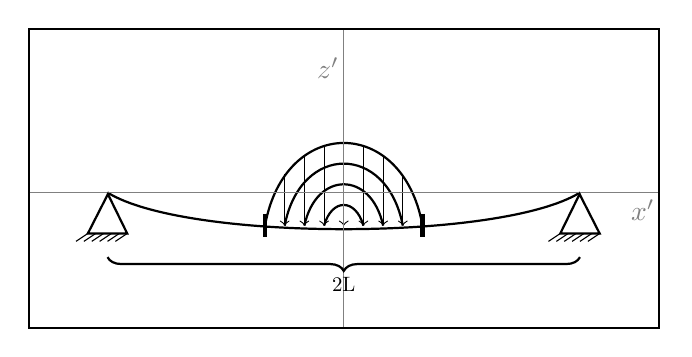
\begin{tikzpicture}
%arrows
\draw [->] (6,1.05) -- (6,0);
\draw [->] (5.75,1) -- (5.75,0);
\draw [->] (6.25,1) -- (6.25,0);
\draw [->] (5.5,0.9) -- (5.5,0);
\draw [->] (6.5,0.9) -- (6.5,0);
\draw [->] (5.25,0.65) -- (5.25,0);
\draw [->] (6.75,0.65) -- (6.75,0);
%parabolas
\draw [thick] (5,0) .. controls (5.25,1.4) and (6.75,1.4) .. (7,0);
\draw [thick] (5.25,0) .. controls (5.45,1.05) and (6.55,1.05) .. (6.75,0);
\draw [thick] (5.5,0) .. controls (5.65,0.7) and (6.35,0.7) .. (6.5,0);
\draw [thick] (5.75,0) .. controls (5.85, 0.35) and (6.15, 0.35) .. (6.25,0);
%markers
\draw [ultra thick] (5,0.15) -- (5,-0.15);
\draw [ultra thick] (7,0.15) -- (7,-0.15);
%string
\draw [thick] (3,0.42) .. controls (4,-0.2) and (8,-0.2) .. (9,0.42);
%coordinate system
\draw [gray] (2,0.42) -- (10,0.42);
\node at (5.8,2) [gray] {$z'$};
\draw [gray] (6,-1.3) -- (6,2.5);
\node at (9.8,0.2) [gray] {$x'$};
\draw [thick] [decorate,decoration={brace,amplitude=5pt,mirror,raise=0ex}] (3,-0.4) -- (9,-0.4) node[midway,yshift=-1em, scale=0.75]{2L};
% \node at (8.7,0.5) {$\tau$};
%fixators
\draw [thick] (2.75,-0.1) -- (3.25,-0.1) -- (3.005,0.4) -- cycle;
\draw (2.75, -0.1) -- (2.6, -0.2);
\draw (2.85, -0.1) -- (2.7, -0.2);
\draw (2.95, -0.1) -- (2.8, -0.2);
\draw (3.05, -0.1) -- (2.9, -0.2);
\draw (3.15, -0.1) -- (3, -0.2);
\draw (3.25, -0.1) -- (3.1, -0.2);
\draw [thick] (8.75,-0.1) -- (9.25,-0.1) -- (8.995,0.4) -- cycle;
\draw (8.75, -0.1) -- (8.6, -0.2);
\draw (8.85, -0.1) -- (8.7, -0.2);
\draw (8.95, -0.1) -- (8.8, -0.2);
\draw (9.05, -0.1) -- (8.9, -0.2);
\draw (9.15, -0.1) -- (9.0, -0.2);
\draw (9.25, -0.1) -- (9.1, -0.2);
%box
\draw[thick] (2,-1.3) rectangle (10,2.5);
\end{tikzpicture}
%caption
\caption{Schematic representation of the physical problem} \label{fig:Schematics}
\end{figure}

\subsection{Governing equations}
We follow \cite{Galeano-RiosEtAl2017} and we model the fluid using linearised Navier-Stokes... 







Following \citet{AgueroEtAl2022} we assume the surface elevation of the elastic membrane $\eta'(r',t')$ is governed by
\begin{equation}
    \partial_{t'}\eta' = u'
\end{equation}
\begin{equation}
    \mu\partial_{t'}u' = -\mu g + \tau\kappa(\eta') - p'
\end{equation}
where $u'(r', t')$ is the vertical velocity of the membrane, $\mu$ is the mass per unit area, $g$ is gravity, $\tau$ is the tension, $p'(r',t')$ is the pressure distribution from the impact, and $\kappa(\eta')$ is twice the mean curvature of the membrane, given in axisymmetric coordinates by
\begin{equation}
    \kappa(\eta') = \frac{\partial_{r'r'}\eta'}{[1+(\partial_{r'}\eta')^{2}]^{3/2}}+\frac{\partial_{r'}\eta'}{r'[1+(\partial_{r'}\eta')^{2}]^{1/2}}
\end{equation}
These equations are subject to:

\paragraph{Boundary conditions:}
\begin{align}
    \eta'(L, t') &= 0 \quad &&\forall t' \ge 0 \quad \text{(fixed rim)} \label{eq:bc_rim} \\ 
    \partial_{r'}\eta'(0, t') &= 0 \quad &&\forall t' \ge 0 \quad \text{(axisymmetry)} \label{eq:bc_sym}
\end{align}

\paragraph{Initial conditions ($t'=0$):}
\begin{align}
    u'(r', 0) &= 0 \quad &&\forall r' \in [0, L] \quad \text{(at rest)} \label{eq:ic_u} \\
    p'(r', 0) &= 0 \quad &&\forall r' \in [0, L] \quad \text{(no pressure)} \label{eq:ic_p} \\
    \tau\kappa(\eta'(r', 0)) &= \mu g \quad &&\forall r' \in [0, L] \quad \text{(equilibrium shape)} \label{eq:ic_shape}
\end{align}

Moreover, the movement of the center of mass of the sphere $h'(t')$ is governed by Newton's second law, that is
\begin{equation}
    \partial_{t'}h' = v'
\end{equation}

\begin{equation}
    m \partial_{t'}v' = -mg + 2\pi \int_{0}^{r_c'(t')} p'(r', t') r' dr'
\end{equation}

where $A(t')$ is the contact area, assumed to be a disk of radius $r_c'(t')$. These are subject to:

\paragraph{Initial conditions ($t'=0$):}
\begin{align}
    h'(0) &= R' + \eta'(0, 0) \quad &&\text{(starts at contact)} \label{eq:ic_h} \\
    v'(0) &= -U'_0 \quad &&\text{(initial velocity)} \label{eq:ic_v}
\end{align}

\paragraph{Compatibility conditions for deformation:} 
To couple the motion of the sphere and the membrane, a set of compatibility conditions, known as the **kinematic match**, are imposed on the contact area $A(t')$ and its boundary $L(t')$:
\begin{enumerate}
    \item The surfaces must coincide on the contact area:
    \begin{equation}
        \eta'(r', t') = h'(t') + s'(r') \quad \forall r' \le r_c'(t') 
    \end{equation}
    
    where $s'(r') = -\sqrt{R'^2 - r'^2}$ is the shape of the sphere's lower hemisphere.
    
    \item The vertical velocities must match on the contact area:
    \begin{equation}
        u'(r', t') = v'(t') \quad \forall r' \le r_c'(t')
    \end{equation}
    
    \item The membrane must be tangential to the sphere at the boundary of the contact area:
    \begin{equation}
        \partial_{r'}\eta'(r_c'(t'), t') = s'^{\prime}(r_c'(t'))
    \end{equation}
    
    \item There is no superposition of the surfaces outside the contact area:
    \begin{equation}
        \eta'(r', t') < h'(t') + s'(r') \quad \forall r' > r_c'(t')
    \end{equation}
    
\end{enumerate}

\subsection{Finite differences}
Describe finite difference schemes used.


To accurately capture the spatio-temporal dependence of the pressure distribution, particularly the moving boundary of the contact area $r_c'(t')$, we adopt an Arbitrary Lagrangian-Eulerian (ALE) formulation. This approach uses a time-dependent system of spatial coordinates $X$ that allows the mesh to deform continuously. This ensures that the boundary of the contact area can be precisely tracked, ideally laying on the boundary of an element at all times.

\subsection{Finite differences in time}
For the temporal discretization of the ALE equations, we use a variable-step Backward Difference Formula scheme of order 2 (VS-BDF2) to approximate the temporal derivatives. This is implemented for all time steps except the first, which uses an implicit Euler method. This scheme allows for adaptive time-stepping, which is tuned to guarantee a minimal time-resolution for tracking the boundary of the pressed area.

\subsection{Variational formulation}
We introduce the weak form of the ALE governing equations to develop a variational formulation. This is done by multiplying the governing partial differential equations by a test function $h(x)$ and integrating over the spatial domain $[0,L]$. The resulting residuals must be zero for all test functions, which forms the basis for the finite element implementation.

\subsection{Finite Element Method}
The problem is solved using the Finite Element Method (FEM). The numerical approximations for the membrane elevation $\eta$, vertical velocity $u$, and other variables are expanded on a set of basis functions $h_i(x)$ (e.g., Lagrange polynomials). This expansion is substituted into the weak form, and Galerkin's method is applied, using the basis functions as the test functions.

\subsection{Methods of spines}
To manage the mesh evolution required by the ALE formulation, we implement the method of spines. This technique allows the structured moving mesh to deform continuously along predefined paths (spines). This implementation is key to guaranteeing that the boundary of the contact area remains on an element boundary at all times of interest, which is the key feature for accurately capturing the dynamic load.

\lipsum[5]
\begin{equation}
	\xi _{ij}(t)=P(x_{t}=i,x_{t+1}=j|y,v,w;\theta)= {\frac {\alpha _{i}(t)a^{w_t}_{ij}\beta _{j}(t+1)b^{v_{t+1}}_{j}(y_{t+1})}{\sum _{i=1}^{N} \sum _{j=1}^{N} \alpha _{i}(t)a^{w_t}_{ij}\beta _{j}(t+1)b^{v_{t+1}}_{j}(y_{t+1})}}
\end{equation}

\subsubsection{Headings: third level}
\lipsum[6]

\paragraph{Paragraph}
\lipsum[7]



\section{Examples of citations, figures, tables, references}
\label{sec:others}

\subsection{Citations}
Citations use \verb+natbib+. The documentation may be found at
\begin{center}
	\url{http://mirrors.ctan.org/macros/latex/contrib/natbib/natnotes.pdf}
\end{center}

Here is an example usage of the two main commands (\verb+citet+ and \verb+citep+): Some people thought a thing \citep{kour2014real, hadash2018estimate} but other people thought something else \citep{kour2014fast}. Many people have speculated that if we knew exactly why \citet{kour2014fast} thought this\dots

\subsection{Figures}
\lipsum[10]
See Figure \ref{fig:fig1}. Here is how you add footnotes. \footnote{Sample of the first footnote.}
\lipsum[11]

\begin{figure}
	\centering
	\fbox{\rule[-.5cm]{4cm}{4cm} \rule[-.5cm]{4cm}{0cm}}
	\caption{Sample figure caption.}
	\label{fig:fig1}
\end{figure}

\subsection{Tables}
See awesome Table~\ref{tab:table}.

The documentation for \verb+booktabs+ (`Publication quality tables in LaTeX') is available from:
\begin{center}
	\url{https://www.ctan.org/pkg/booktabs}
\end{center}


\begin{table}
	\caption{Sample table title}
	\centering
	\begin{tabular}{lll}
		\toprule
		\multicolumn{2}{c}{Part}                   \\
		\cmidrule(r){1-2}
		Name     & Description     & Size ($\mu$m) \\
		\midrule
		Dendrite & Input terminal  & $\sim$100     \\
		Axon     & Output terminal & $\sim$10      \\
		Soma     & Cell body       & up to $10^6$  \\
		\bottomrule
	\end{tabular}
	\label{tab:table}
\end{table}

\subsection{Lists}
\begin{itemize}
	\item Lorem ipsum dolor sit amet
	\item consectetur adipiscing elit.
	\item Aliquam dignissim blandit est, in dictum tortor gravida eget. In ac rutrum magna.
\end{itemize}


\bibliographystyle{unsrtnat}
\bibliography{references}  %%% Uncomment this line and comment out the ``thebibliography'' section below to use the external .bib file (using bibtex) .


%%% Uncomment this section and comment out the \bibliography{references} line above to use inline references.
% \begin{thebibliography}{1}

% 	\bibitem{kour2014real}
% 	George Kour and Raid Saabne.
% 	\newblock Real-time segmentation of on-line handwritten arabic script.
% 	\newblock In {\em Frontiers in Handwriting Recognition (ICFHR), 2014 14th
% 			International Conference on}, pages 417--422. IEEE, 2014.

% 	\bibitem{kour2014fast}
% 	George Kour and Raid Saabne.
% 	\newblock Fast classification of handwritten on-line arabic characters.
% 	\newblock In {\em Soft Computing and Pattern Recognition (SoCPaR), 2014 6th
% 			International Conference of}, pages 312--318. IEEE, 2014.

% 	\bibitem{hadash2018estimate}
% 	Guy Hadash, Einat Kermany, Boaz Carmeli, Ofer Lavi, George Kour, and Alon
% 	Jacovi.
% 	\newblock Estimate and replace: A novel approach to integrating deep neural
% 	networks with existing applications.
% 	\newblock {\em arXiv preprint arXiv:1804.09028}, 2018.

% \end{thebibliography}


\end{document}
